\documentclass[tikz,border=5pt]{standalone}
\usepackage{helvet}
\usepackage{amsmath}
\renewcommand{\familydefault}{\sfdefault}
\usetikzlibrary{arrows.meta,positioning,fit}

\definecolor{posc}{RGB}{ 30,130, 70}
\definecolor{negc}{RGB}{190, 55, 45}
\definecolor{obsc}{RGB}{110,110,110}

\begin{document}
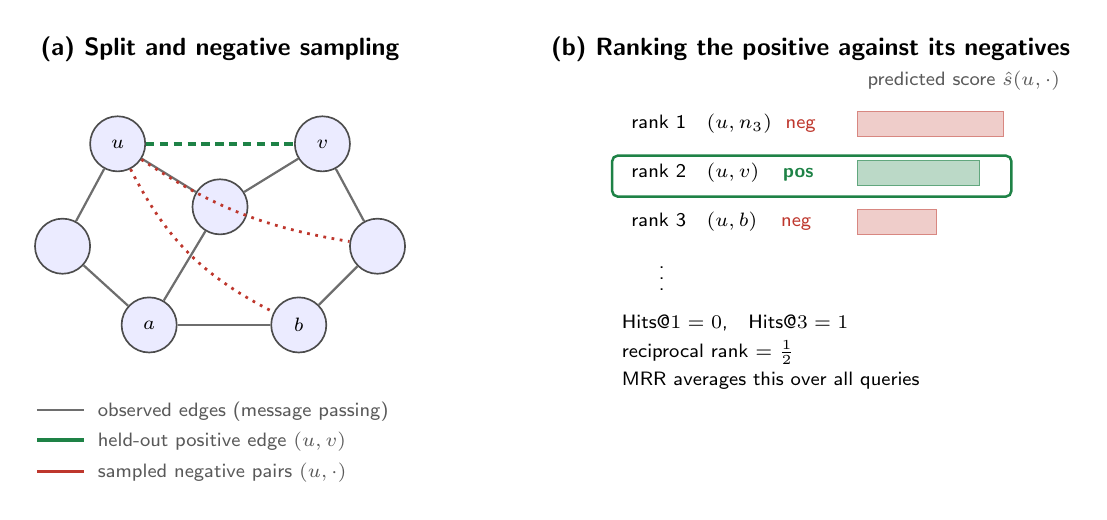
\begin{tikzpicture}[
  font=\small,
  v/.style={circle, draw=black!70, fill=blue!8, line width=0.6pt,
            minimum size=7mm, inner sep=0pt, font=\scriptsize\bfseries},
  obsedge/.style={draw=obsc, line width=0.8pt},
  posedge/.style={draw=posc, line width=1.3pt, dash pattern=on 3pt off 2pt},
  negedge/.style={draw=negc, line width=1.0pt, dotted},
  ttl/.style={font=\small\bfseries, align=center},
  sub/.style={font=\scriptsize, align=center, text=black!65},
  lbl/.style={font=\scriptsize, align=left},
]

% ---------------- left: the graph with held-out edges ----------------
\node[ttl] at (2.3,3.5) {(a) Split and negative sampling};

\node[v] (u) at (1.0,2.3) {$u$};
\node[v] (v) at (3.6,2.3) {$v$};
\node[v] (n1) at (0.3,1.0) {};
\node[v] (n2) at (2.3,1.5) {};
\node[v] (n3) at (4.3,1.0) {};
\node[v] (a)  at (1.4,0.0) {$a$};
\node[v] (b)  at (3.3,0.0) {$b$};

% observed (message-passing / training) edges
\draw[obsedge] (u)--(n1); \draw[obsedge] (u)--(n2); \draw[obsedge] (n2)--(v);
\draw[obsedge] (v)--(n3); \draw[obsedge] (n1)--(a); \draw[obsedge] (a)--(n2);
\draw[obsedge] (n3)--(b); \draw[obsedge] (a)--(b);

% held-out positive
\draw[posedge] (u)--(v);
% sampled negatives
\draw[negedge] (u) to[bend right=18] (b);
\draw[negedge] (u) to[bend right=12] (n3);

\node[sub, align=left, anchor=north west] at (-0.15,-0.85)
  {\textcolor{obsc}{\rule[0.6ex]{6mm}{0.8pt}}~~observed edges (message passing)\\[1.1mm]
   \textcolor{posc}{\rule[0.6ex]{6mm}{1.3pt}}~~held-out positive edge $(u,v)$\\[1.1mm]
   \textcolor{negc}{\rule[0.6ex]{6mm}{1.0pt}}~~sampled negative pairs $(u,\cdot)$};

% ---------------- right: the induced ranking ----------------
\begin{scope}[xshift=7.4cm]
  \node[ttl] at (2.4,3.5) {(b) Ranking the positive against its negatives};

  \def\rowy{2.55}
  \node[lbl, anchor=west] at (0.0,\rowy)        {rank 1\quad $(u,n_3)$\ \ \textcolor{negc}{neg}};
  \node[lbl, anchor=west] at (0.0,{\rowy-0.62}) {rank 2\quad $(u,v)$\ \ \ \,\textcolor{posc}{\textbf{pos}}};
  \node[lbl, anchor=west] at (0.0,{\rowy-1.24}) {rank 3\quad $(u,b)$\ \ \ \,\textcolor{negc}{neg}};
  \node[lbl, anchor=west] at (0.0,{\rowy-1.86}) {\ \ \ \ $\vdots$};

  % score bars
  \draw[fill=negc!25, draw=negc!60] (3.0,{\rowy-0.16}) rectangle ++(1.85,0.32);
  \draw[fill=posc!30, draw=posc!70] (3.0,{\rowy-0.78}) rectangle ++(1.55,0.32);
  \draw[fill=negc!25, draw=negc!60] (3.0,{\rowy-1.40}) rectangle ++(1.00,0.32);
  \node[sub, anchor=west] at (3.0,{\rowy+0.55}) {predicted score $\hat{s}(u,\cdot)$};

  % highlight the positive row
  \draw[posc, line width=0.9pt, rounded corners=2pt]
       (-0.12,{\rowy-0.92}) rectangle (4.95,{\rowy-0.40});

  \node[lbl, anchor=west, text width=5.4cm] at (-0.12,{\rowy-2.9})
    {$\text{Hits@}1 = 0$,\quad $\text{Hits@}3 = 1$\\[0.8mm]
     reciprocal rank $=\tfrac{1}{2}$\\[0.8mm]
     MRR averages this over all queries};
\end{scope}

\end{tikzpicture}
\end{document}
